\scanpage{129}
\margin{\handwritten{\uline{NB}} \uline{Que\deleted{\unsure{e|o}}stion} Sous réserve $B$ associative unitaire, si $A$ est commutative, $B$ l'est-elle aussi ? (On suppose $A$ associative unitaire). Question analogue quand on a des structures graduées avec antic\deleted{q}ommutativité. Donc, la condition de \deleted{symé} comp. aux sym. pour un $c$ est-elle surabondante, en prés. des autres com\deleted{d}pat\handwritten{\unsure{ab|b}.} ?\begin{tikzpicture}[x=.35cm,y=.35cm,baseline=-.6ex]\draw (.45,.2) .. controls (-.1,-.2) and (-.3,-2.6) .. (.2,-3.3) .. controls (.9,-4) and (2,-3.2) .. (4,-3.1);\end{tikzpicture}}
de base fidèlement plat $k\handwritten{\longrightarrow}B$, \deleted{le foncteur} il devient trivial, donc on a un ``torseur'' sous le monoïde $\unsure{\deleted{G}H|\mathbb H|\mathbb G}_{k'}$ ; alors le nouveau foncteur fibre $G$ est déduit de $F'=F\otimes_k k'$ par torsion à l'aide de $G$ \ldots

Mais supposons seu\deleted{\unsure{o|e}}lement $A$ algèbre associative unitaire, et $B$ itou, sans condition de commutativité.\inserted{On suppose $A$ avec \uline{antipodisme}\inserted{\handwritten{$\underline{a}$}} (s'en passer ?).}\handwritten{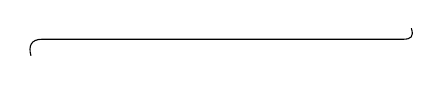
\begin{tikzpicture}[x=.35cm,y=.35cm,baseline=-.2ex]\draw (0,-.5) .. controls (-.1,-.15) and (0,.1) .. (.4,.1)--(13.5,.1) .. controls (13.8,.1) and (13.9,.2) .. (13.8,.5);\end{tikzpicture}} Donnons-nous un $\handwritten{\sigma\in}U\otimes_k U$ \deleted{ci-des} comme ci-dessus pour introduire une relation de commutativité $\handwritten{\unsure{\psi|\phi}}$ . Notons (qu'à celà près que $k'$ n'est plus supposé un corps) on trouve une catégorie $C'=C\otimes_k k'$ sur $k'$, avec $\otimes$, définie\inserted{\handwritten{(soit par $U'$, \uuline{soit} \unsure{dual.|duaux.|deux.})}}\handwritten{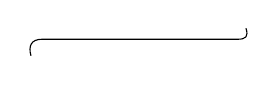
\begin{tikzpicture}[x=.35cm,y=.35cm,baseline=-.2ex]\draw (0,-.5) .. controls (-.1,-.15) and (0,.1) .. (.4,.1)--(7.5,.1) .. controls (7.8,.1) and (7.9,.2) .. (7.8,.5);\end{tikzpicture}} par le ``proanneau'' $V=G(U)=L\handwritten{\unsure{\overset{\uparrow}{\overset{\Delta}{\otimes}}|\overset{\uparrow}{\widehat{\otimes}}}}_U(U,\mathrm{int})$, où $(U,\mathrm{int})$ désigne $U$ muni de la structure de $U$-module \deleted{(donc de pro-objet de} (et même d'objet``pro-anneau'' (pour $\otimes$) de $C$) défini à l'aide de sa structure de bimodule sur $U^o\overset{\handwritten{\scriptscriptstyle\wedge}}{\otimes} U$ \deleted{à l'aide de} par restriction des scalaires via $U\handwritten{\xrightarrow{\Delta}}U\overset{\handwritten{\scriptscriptstyle\wedge}}{\otimes} U\handwritten{\xrightarrow{\underline a\otimes\mathrm{id}_U}}U^o\overset{\handwritten{\scriptscriptstyle\wedge}}{\otimes} U$ : Tordant par $L$ et utilisant le fait que l'on a une compatibilité avec $\otimes$, on trouve un pro-anneau $V$ sur $k'$, et ce dernier hérite de $U$ une application diagonale \ldots
\margin{\handwritten{?}}
\margin{\handwritten{a) donner un sens intrinsèque : $C\otimes_k k'$, indépendamment de \deleted{$\unsure{\circ|a|\otimes}$} la donnée de $F$ (\uline{NB} si $k'$ n'est pas un corps, ce n'est pas une catégorie \uline{abélienne}, seulement additive)}}
Ceci\deleted{\unsure{,|r|s|x}} dit, si on a une donnée $\handwritten{\sigma\in}U\overset{\handwritten{\scriptscriptstyle\wedge}}{\otimes} U$ satisfaisant les conditions (1)\inserted{plus haut,}\handwritten{\begin{tikzpicture}[x=.35cm,y=.35cm,baseline=-.2ex]\draw (0,-.5) .. controls (-.1,-.15) and (0,.1) .. (.4,.1)--(4.5,.1) .. controls (4.8,.1) and (4.9,.2) .. (4.8,.5);\end{tikzpicture}} peut-on définir en termes de $\handwritten{\sigma}$ (ou existe-t-il tout au moins) un élément $\handwritten{\tau\in}V\overset{\handwritten{\scriptscriptstyle\wedge}}{\otimes}_k V$ satisfaisant les relations analogues à (1), de telle façon que $(G,c)$ soit compatible aux isomorphismes de symét\deleted{\unsure{t|F}}r\deleted{\unsure{r|t}}ie $\handwritten{\psi}$ dans $C$ d\unsure{é|e}fini par $\handwritten{\sigma}$, $\handwritten{\psi'}$ dans $C'$ défini par $\handwritten{\tau}$ ??? La seule chance de \deleted{le montre} construire un $\handwritten{\tau}$ canoniquement semble de prouver que $\handwritten{\tau}$ est ``invariant'' lorsqu'on fait opérer $U$ sur $U\overset{\handwritten{\scriptscriptstyle\wedge}}{\otimes}_k U=(U,\mathrm{int})\overset{\handwritten{\scriptscriptstyle\wedge}}{\otimes}(U,\mathrm{int})$ grâce à son \deleted{\unsure{e|F}}\deleted{\unsure{u|e}}action dite plus haut sur les deux facteurs, ce qui s'exprime par la relation $U^+ .\handwritten{\unsure{\tau^{\scriptscriptstyle\cdot}|\tau'|\tau}}=0$.\inserted{\handwritten{[Vérifier dans le cas gradué ce qui en est !]}}\handwritten{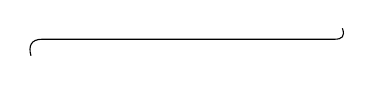
\begin{tikzpicture}[x=.35cm,y=.35cm,baseline=-.2ex]\draw (0,-.5) .. controls (-.1,-.15) and (0,.1) .. (.4,.1)--(11.0,.1) .. controls (11.3,.1) and (11.4,.2) .. (11.3,.5);\end{tikzpicture}} - Si ceci marchait (ce qui améliorerait le résultat souhai\deleted{t}té en NB au haut de la page), cela montrerait que dans l'étude des foncteurs fibres, il y a lieu de laisser tomber les questions de compatibilité aux symétries, celles-ci se récupérant toujours après coup.\inserted{\handwritten{(Mais cf exemples n\textsuperscript{o}1\unsure{2|1}).}}
\margin{\handwritten{b) Montrer qu'une structure $\unsure{\otimes|\ominus}$, éventuellement avec données $\varphi,\psi,1,\unsure{\vee|\nu|\gamma}$. se prolonge automatiquement à $C'$, avec ses axiomes}}
\margin{\handwritten{c) généraliser, pour un foncteur \unsure{complet|compatible|comme} $G:C\to\mathrm{Mod}(k')$, la description du n\textsuperscript{o}6 en description de $C'$ en termes d'un pro-anneau $U'=\mathrm{End}(G)$, et réexpliciter en termes de ce dernier les diverses structures sur $C$: $\otimes,\unsure{\varphi|\rho},\psi,1,\unsure{\vee|\nu}$}}

Il resterait alors la question d'une description \uline{intrinsèque} d'une catégorie $C$ comme dans le n\textsuperscript{o}1,\inserted{\handwritten{avec $\unsure{\overset{\circ}{\times}|\check X}$}}\handwritten{\begin{tikzpicture}[x=.35cm,y=.35cm,baseline=-.2ex]\draw (0,-.5) .. controls (-.1,-.15) and (0,.1) .. (.4,.1)--(2.6,.1) .. controls (2.9,.1) and (3.0,.2) .. (2.9,.5);\end{tikzpicture}} indépendam\deleted{e}m\deleted{\unsure{m|n}}e\deleted{\unsure{e|t}}n\deleted{n}t de la donnée d'un $F$ préli%
